\chapter{Abstract}

For years, heuristic search on automated planning has achieved a significant success and shown its
ability to scale to large problems. Much of the success can be attributed to the development of more
and more sophisticated heuristic functions, while relatively less attention was paid on the 
base search algorithms.

For example, despite the number of papers which try to push the state of the art of the
optimal planning by improving the admissible heuristic functions and developing their theory, much
less focus was put on the common underlying algorithm, A*, until \cite{Asai2016}.  Similarly, while
there is a large body of work on satisficing planning algorithms, many algorithms tend to be ad-hoc
and lack theoretical foundation other than completeness. \sota LAMA planner
\cite{richter2010lama} incorporates 5 improvements at once and the reason of its success in the
planning competition is hard to discuss.

The aim of this dissertation is to provide a unified view for search algorithms and propose new algorithms
based on the new understanding.
% and introduce a new
% tool to analyze those algorithms, namely Fractal Dimension. 
This dissertation proceeds as follows:
In \refsec{sec:opt}, we show that optimal search can be reduced to a sequence of satisficing
searches, so that we can focus on satisficing search only. In \refsec{sec:sat}, we show that a
heuristic satisficing search algorithm is defined by a heuristics, inter-plateau diversification
and intra-plateau diversification, and each strategy reduces to blind search. 
Finally we review some existing work on diversification/blind search strategies,
as well as the ones proposed by us, which can be described in our framework.
% Finally, \refsec{sec:fractal} propose the use of Fractal
% Dimension and ways to analyze existing algorithms.

\section{Optimal Planning as a Sequence of Satisficing Search}

\label{sec:opt}

In the aim of abstracting away the differences between the optimal and satisficing search,
we present an alternative view to optimal search algorithm \astar \cite{asai2017tie}.
 
\astar is a standard search algorithm for finding an optimal cost path from an initial state $s$ to
some goal state $g \in G$ in a search space represented as a graph \cite{hart1968formal}.
It expands the nodes in the best-first order of $f(n)$ up to $f^*$, where $f(n)$ is a lower bound of the
cost of the shortest path that contains a node $n$ and $f^*$ is the cost of the optimal path.

We empirically show that in many combinatorial search problems, the size of the last layer
$f(n)=f^*$ of the search, called a \emph{final plateau}, accounts for a significant fraction of the
effective search space of \astar.  By carefully analyzing search within an $f$-cost plateau, we
developed an effective {\it knowledge-free}, tie-breaking method which diversifies the \emph{depth}
of a node in the current plateau.  The resulting algorithm significantly improves the search
performance on domains with 0-cost actions \cite{Asai2016}. 

Extending the intuition, we proposed a more general framework which underscores the importance of
tie-breaking in \astar: \emph{Cost-optimal search can be seen as a series of satisficing searches on
each plateau}. In this framework, the problem of tie-breaking can be reduced to a
satisficing search.

While \astar requires the first sorting criterion $f$ to use an admissible heuristic in order to
find an optimal solution, there are no requirements on the second or later sorting criteria.
This means that the search within the same $f$ plateau can be an arbitrary satisficing
search without any cost minimization requirement. For example, if we ignore the first sorting
criterion in the standard admissible strategy $[f,h,\fifo]$, which first sort the OPEN list by
$f$-value, then by $h$-value and finally by a First-In-First-Out order, then we have $[h,\fifo]$, which
is exactly the same configuration as a Greedy Best First Search (GBFS) using \fifo default
tie-breaking. This means that within a particular $f$-cost plateau, $[f,h,\fifo]$ is performing a
satisficing GBFS.

% \footnote{This refers to any algorithm which seeks a satisficing solution, as opposed to the
% ``satisficing'' track setting in IPC which also seeks to minimize the plan cost with anytime
% algorithms}

From this perspective, we can reinterpret \astar as follows: \astar expands the
nodes in the best-first order of $f$ value. When the heuristic function is admissible, the $f$ values of
the nodes expanded by \astar never decreases during the search process.  Thus, the entire process of
\astar can be considered as a series of search episodes on each $\plateau{f}$.  The search on each
plateau terminates when the plateau is proven to contain no goal nodes (UNSAT), or when a goal is
found (SAT).  When the plateau is UNSAT, then the search continues to the plateau with the next
smallest $f$ value.

% \begin{algorithm}
%  \begin{algorithmic}
%   \LOOP
%   \STATE Search $\plateau{f}$ for any goal state, using satisficing search algorithm
%   \IF{$\plateau{f}$ contains some goal (Plateau is SAT)}
%   \RETURN solution
%   \ELSE
%   \STATE Increase $f$ 
%   \ENDIF
%   \ENDLOOP
%  \end{algorithmic}
%  \caption{Reinterpretation of \astar as iterations of satisficing search on plateaus}
%  \label{alg:astar-sat}
% \end{algorithm}

Using this understanding, we empirically evaluate the performance of \astar on zero-cost domains,
using an inadmissible FF heuristics \cite{Hoffmann01} for a tiebreaking criterion (the second
sorting criteria) and show that it improves the performance. Since the primary (first) sorting
criterion is admissible, using the inadmissible criterion for tiebreaking does not affect the
optimality of the solution. This opens up the opportunity to use even larger variety of satisficing
search algorithms as a mean of searching the plateaus in \astar search.

\section{Diversified Satisficing Planning}

\label{sec:sat}

To further abstract away the differences between various algorithms, we unified the extensions for
Greedy Best First Search, the mainstream satisficing search algorithm. We particularly focused on
\emph{diversified search} and \emph{plateau-escaping}.

Diversified search \cite{imai2011novel,valenzano2014comparison,xie14type}, in satisficing setting,
has been commonly referred to a group of algorithms that extends GBFS and does not strictly obey the
best-first order of heuristic values. The method for diversifying the search may vary
across algorithms.

Plateau escaping has numerous synonyms. Firstly, it is equivalent to tie-breaking
methods because it operates within the same heuristic plateau defined as a set of search nodes
sharing the same $h$-value. Another name for this group of algorithms is \emph{local exploration}
\cite{XieMH15,XieH14gbfsle}. Despite the name, it does not necessarily search any
particular neighborhood defined by the distance measure. The term \emph{plateau escaping} is used in
the work by Enforced Hill Climbing \cite{Hoffmann01} and Marvin planner \cite{Coles07}.

We merged these two notions into \emph{inter-plateau} and \emph{intra-plateau} diversification
strategies, and showed their algorithmic and empirical orthogonality \cite{Asai2017b}. Notably, each
strategy is defined as a knowledge-free, blind search strategy. This effectively generalizes various
satisficing heuristic forward-search algorithms: Each algorithm consists of a heuristic function,
inter-plateau strategy and intra-plateau strategy. For example, GBFS using FF heuristics is defined
by the FF heuristics, Best-First inter-plateau strategy and an arbitrary tiebreaking strategy (such
as blind breadth-first search).

% However, we do not claim that these notions always cover every algorithms, such as the heuristic
% search with complex open list operations (e.g. alternating or pareto open list \cite{RogerH10}).

\section{Diversification Strategies}

\label{sec:div}

As it was shown that a heuristic search algorithm can be characterized by its three components, and
the two modes of diversification are both blind search variants, we can focus only on the
characteristics of blind search.  As the baseline, Breadth-first, Depth-first and Random search
respectively correspond to FIFO, LIFO and Random order strategy for selecting a node from the OPEN
list in blind search.

\subsection{Type/Depth-Based Diversification}

The notions of inter-vs-intra plateau diversification allows us to discuss and compare depth
diversification \cite{Asai2016} and Type-GBFS \cite{xie14type} within a unified framework -- it
turns out that these are essentially the same algorithm, except that they are using different key
values (metrics) in different contexts (inter-vs-intra plateau, satisficing-vs-optimal search).

\cite{lelis2013stratified} define a general framework for
adding exploration to search using ``type systems'', and \cite{xie14type} proposed a node selection technique based on type systems:

\begin{defi} 
A \emph{Type system} \cite{lelis2013stratified} is a 
function from a node to a vector,
$T: \text{node} \rightarrow \mathbb{Z}^k, T(n)=\brackets{t_1(n) \ldots t_k(n)} $, where each function $t_i(n)$ returns an integer for each node $n$.
\end{defi}

\begin{defi}
% \emph{Type-Based Diversification} 
 \emph{Type-Based Node Selection} \cite{xie14type}
with a type system $T(\cdot)$ of $k$ types maintains a $k$-dimensional matrix of sets of nodes,
 where each set $S_v$ is associated with a vector $v=\brackets{v_1,\ldots,v_k}$.
 Each node $n$ is stored in $S_{T(n)}$.
 For dequeueing, it randomly selects a non-empty set from all sets,
 and a random node in the set is dequeued.
\end{defi}

% The reason for selecting a set at random is to try to allocate the search effort among a diverse set of nodes.
% Some sets could contain a large number of nodes while others are only scarcely populated.
% Type-based node selection tries to remove this cardinality bias among buckets.
% Because type-based node selection  has this diversification as an explicit goal and is best understood as a diversification strategy, we call it \textbf{\emph{type-based diversification}} in the rest of this paper.

% % describe Type-GBFS first to keep the description of all the type-based previous work together.
Type-GBFS \cite{xie14type} uses type-based diversification with type system $\brackets{g,h}$ for
inter-plateau exploration. Their inter-plateau exploration is implemented by queue alternation
\cite{RogerH10} between standard Best-First queue and type-based diversification queue.

Depth diversification \cite{Asai2016} % originally addressed the issue of zero-cost actions in
% admissible search with \astar, and it 
uses Type-based node selection with plateau depth $\depth$ for
intra-plateau diversification, where $\depth$ is a number of steps from the last node $n'$ to the
current node $n$ with $h(n')<h(n)$, along the path from the initial state through parent pointers.
% % 
% In order to use $\depth$ for GBFS, the resulting configuration is $[h,\depth]$, and the depth $d$ is
% defined for each $h$-plateau.  This configuration is considered as an instance of intra-plateau
% type-based diversification because it uses type-based diversification with type system $\depth$ for
% diversifying the search within plateaus defined by $h$.

\subsection{Invasion Percolation Diversification}

A limitation of type-based diversification based on path distance is that it does not diversify with
respect to breadth -- nodes with equal estimated distance from goals ($h$), initial states ($g$) or
plateau entrance ($d$) are put in a single set.  This makes it susceptible to pathological behavior
on graphs where some nodes have many more children than others.


\begin{figure}[hbt]
   \centering
 \begin{minipage}{3.25in}
   \centering
 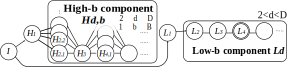
\includegraphics{img/model3.pdf}
 \caption{Example case exhibiting large bias in the branching factor depending on the subgraph.}
 \label{fig:model}
 \end{minipage}
\begin{minipage}{3.25in}
  \centering
 \includegraphics[width=0.5\linewidth]{img/static/ip.png}
 \caption{Invasion Percolation on 2-dimensional lattice}
 \label{fig:ip}
\end{minipage}
\end{figure}

Consider a blind search on a directed acyclic graph
shown in \refig{fig:model}.
The graph consists of two large components, \textbf{high-b} and \textbf{low-b} branches, and their entries $H_1,L_1$. The initial search node is $I$ and the goal node is $L_4$.
Both branches have maximum depth $D$, and the high-b branch has maximum width $B$.
Both $B$ and $D$ are very large.
This graph presents a pathological case for all of the previously described methods (\lifo, \fifo, \ro and type-based diversification), depending on successor ordering.
\lifo performs a DFS, and if \lifo first searches $H_1$ and the high-b branch due to successor ordering, it must explore the entire high-b branch before expanding $L_1$ and low-b branch.
\fifo performs Breadth-First Search (BreadthFS), and  will therefore suffer from the  high branching factor at depth 2 of the high-b branch, getting stuck before reaching $L_4$.
Although randomization can allow \ro to be better off than the behavior of \fifo/BreadthFS, the effect is limited:
For example, while expanding depth 2, \ro may occasionally expand depth 3 because it uniformly randomly selects a node from OPEN.
However, the probability of expanding nodes at depth 3 is initially only $1/(B+1)$ and continues to be small until  most of the nodes at depth 2 are expanded, 
because OPEN is mostly populated with the nodes from depth 2.
Depth-based diversification addresses the depth bias of BreadthFS.
However, even though it distributes the effort among various depths,
the probability of expanding $L_2,L_4$ at depths 2 and 4, is only $1/(B+1)$ each, which is very low when $B$ is very large.


We proposed \emph{Invasion Percolation-based diversification (IP-diversification)}, a
diversification strategy for satisficing search that addresses this type of bias \cite{Asai2017b}.
IP-diversification combines randomization and Prim's method \cite{prim1957shortest} for Minimum
Spanning Tree (MST).
% 
Invasion Percolation \cite{wilkinson1983invasion} simulates the distribution of fluid slowly
invading porous media, e.g., water replacing the air in a porous rock.  We focus on a variant called
bond IP (BIP), where ``bonds'' indicate edges in a lattice, and present the graph-based description
by \cite{barabasi1996invasion}.
% 
Given initial node(s) and a graph whose edges are assigned independent random values, BIP
iteratively marks the nodes.  Once assigned, the random value on each edge never changes.
The initial nodes are marked by default.  In each iteration marks an unmarked node to which the
least-value outgoing edge leads.  Marked nodes represent the porous sites whose air is replaced by
the water (invader).

% \citeauthor{barabasi1996invasion} (\citeyear{barabasi1996invasion}) showed
% that this algorithm is equivalent to applying Prim's method for MST \cite{prim1957shortest} on a
% randomly weighted graph: Prim's method constructs an MST by iteratively adding a neighboring edge
% with the least edge costs to the existing tree.

\refig{fig:ip} illustrates a 2-D lattice after running BIP for a while. The initial nodes are at the
leftmost edge of the rectangular region, i.e. the fluid percolates from the left. The resulting
structure has holes of various sizes that the fluid has not invaded, due to the high-valued edges
surrounding the neighbors of the holes, which serve as an embankment preventing the water from
invading. Since the random value on each edge is fixed, the algorithm does not mark the nodes inside
the hole until it marks all nodes with smaller random values in the entire space outside the
embankments.  This behavior is critical to forming a fractal structure.

% This strategy, used for either or both of intra and inter-plateau diversification, improves the
% performance of GBFS as well as \sota planner FD/LAMA2011 \cite{Asai2017b}.


